\documentclass[../practica_01.tex]{subfiles}

\begin{document}

    \begin{itemize}
        \item $A = (1,2,3)$
        \item $B = (1,3,6)$
        \item $C = (3,8,6)$
        \item $D = (3,7,3)$
        \item $\overrightarrow{u} = B - A = (0,1,3) $
        \item $\overrightarrow{v} = C - A = (2,6,3) $
    \end{itemize}

    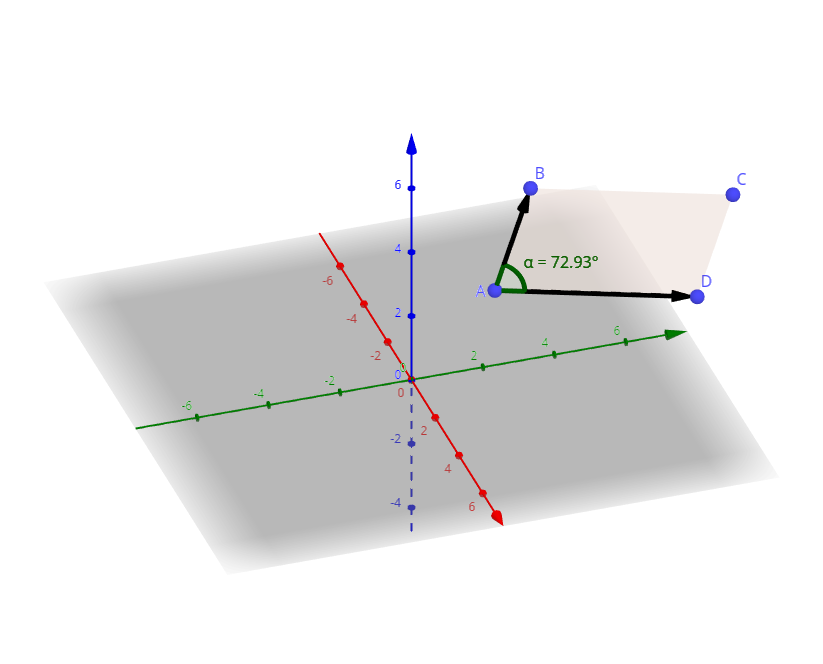
\includegraphics[scale=0.4]{ej12/resources/ej12.png} $ $

    $Area = \norm*{\overrightarrow{u} \cross \overrightarrow{v}} = $
    $\norm*{(0,1,3) \cross (2,6,3)}$

    $ $

    $\begin{vmatrix}
        i & j & k \\
        0 & 1 & 3 \\
        2 & 6 & 3
    \end{vmatrix}$

    $= (1 \cdot 3) - (6 \cdot 3)) \cdot \widehat{i}$
    $- (0 \cdot 3) - (2 \cdot 3)) \cdot \widehat{j}$
    $+ (0 \cdot 6) - (2 \cdot 1)) \cdot \widehat{k} = $
    $ (-15, 6, -2) $

    $\norm*{(-15, 6, -2)} = \sqrt{(-15)^2+6^2+(-2)^2} = $
    $\sqrt{225+36+4} = \sqrt{265} $

\end{document}